\documentclass[11pt,a4paper]{article}

\usepackage[utf8]{inputenc}
\usepackage[T1]{fontenc}
\usepackage{lmodern}
\usepackage[french]{babel}
\usepackage[margin=2.3cm]{geometry}
\usepackage{amsmath}
\usepackage{graphicx}
\usepackage{booktabs}
\usepackage{siunitx}
\usepackage{xcolor}
\usepackage{listings}
\usepackage{enumitem}
\usepackage{newunicodechar}
\usepackage{microtype}
\emergencystretch=2em
\newunicodechar{→}{\ensuremath{\to}}
\newunicodechar{œ}{\oe}
\usepackage[colorlinks=true,linkcolor=blue!50!black,citecolor=blue!50!black,urlcolor=blue!50!black]{hyperref}

\sisetup{locale=FR, group-minimum-digits=4}
\graphicspath{{../benchmark/results/}}
\setlist{itemsep=2pt}

\lstset{basicstyle=\ttfamily\small, columns=fullflexible, frame=single,
        backgroundcolor=\color{gray!8}, rulecolor=\color{gray!40},
        keepspaces=true, showstringspaces=false, breaklines=true,
        literate={é}{{\'e}}1 {è}{{\`e}}1 {à}{{\`a}}1 {ç}{{\c c}}1}

\newcommand{\rscan}{r\textsuperscript{2}SCAN}

\title{VASP sur GPU\\[4pt]
\large Ce qui accélère un calcul, ce qui ne l'accélère pas,\\
et comment utiliser au mieux les deux H100 de vm1-ic2mp}
\author{Gilles Frapper \\ Professeur des Universités, Chimie Théorique \\
IC2MP UMR 7285 CNRS, Université de Poitiers \\
\href{mailto:gilles.frapper@univ-poitiers.fr}{gilles.frapper@univ-poitiers.fr}}
\date{2 octobre 2026}

\begin{document}
\maketitle

\begin{abstract}
Ce rapport rassemble, sous forme pratique, les enseignements des campagnes de mesure menées
du 26 septembre au 2 octobre 2026 avec VASP 6.5.1 (version GPU OpenACC) sur le nœud
vm1-ic2mp (2 × NVIDIA H100 NVL). Plus de 350 calculs ont été analysés, sans compter les phonons : points simples et
optimisations PBE et \rscan{} de 1 à 64 atomes sur 1 et 2 GPU, phonons, calculs simultanés
sur une GPU avec et sans MPS, dynamique moléculaire de LiN\textsubscript{3} (144 atomes),
et deux campagnes consacrées au paramètre \texttt{NSIM} jusqu'à 216 atomes, en PBE et HSE06.
Le message principal est simple : jusqu'à une centaine d'atomes, un calcul VASP n'occupe
qu'une petite partie d'une H100. Les leviers efficaces ne sont pas les réglages fins de
l'INCAR (\texttt{NSIM} n'apporte rien : $\pm$\SI{5}{\percent}), mais l'organisation des
calculs : un calcul par GPU plutôt qu'un calcul sur deux GPU, et plusieurs calculs sur la même
GPU sous MPS, ce qui multiplie le débit par 2,5 à 5,8.
\end{abstract}

\section*{L'essentiel en une page}
\addcontentsline{toc}{section}{L'essentiel en une page}

\begin{center}
\small
\begin{tabular}{@{}p{0.36\linewidth}p{0.58\linewidth}@{}}
\toprule
Question & Réponse mesurée sur vm1-ic2mp \\
\midrule
Un calcul de 1 à 64 atomes remplit-il une H100 ? &
Non. Utilisation moyenne de 10 à \SI{50}{\percent}, mémoire de 2,8 à \SI{12,2}{Go} sur 94.
Vers 150--200 atomes, l'utilisation monte à 64--\SI{75}{\percent}. \\
\addlinespace
Faut-il deux GPU pour un calcul ? &
Rarement. Gain de 1,0 à 1,9$\times$ seulement. Deux calculs indépendants, un par GPU,
donnent plus de débit. \\
\addlinespace
Sur deux GPU, \texttt{KPAR} = 1 ou 2 ? &
\texttt{KPAR} = 2 dès qu'il y a plus de 4 points k (42 cas sur 56) ;
\texttt{KPAR} = 1 seulement avec 3--4 points k et des mailles de 64 atomes. \\
\addlinespace
Faut-il augmenter \texttt{NSIM} ? &
Non. De 4 à 128 : au mieux $+$\SI{6}{\percent}, souvent rien, et jusqu'à
$-$\SI{5}{\percent} avec $+$\SI{27}{Go} de mémoire pour Si 216 atomes à \texttt{NSIM} = 128.
Garder la valeur par défaut ou 8--32. \\
\addlinespace
Plusieurs petits calculs à la fois ? &
Oui, \textbf{mais uniquement sous MPS} : débit $\times$4 à 5,8 avec 8 calculs par GPU.
Sans MPS, le lot est jusqu'à 1,8 fois \emph{plus lent} que les calculs en série. \\
\addlinespace
\texttt{vasp\_gam} pour le point $\Gamma$ ? &
Gain modeste : \SI{10}{\percent} de temps et \SI{27}{\percent} de mémoire GPU en moins
(AIMD LiN\textsubscript{3}, 144 atomes). \\
\addlinespace
Combien coûtent \rscan{} et HSE06 ? &
\rscan{} : 1,6 à 8$\times$ PBE en point simple, jusqu'à 16$\times$ en optimisation.
HSE06 : environ 60$\times$ PBE par pas électronique (MgO, 32 atomes). \\
\addlinespace
Les résultats sont-ils fiables ? &
Oui. Temps reproductibles à \SI{1}{\percent} ; énergies identiques sur 1 et 2 GPU
(\SI{0,01}{meV/atome}) et quel que soit \texttt{NSIM}. \\
\bottomrule
\end{tabular}
\end{center}

\tableofcontents

% ---------------------------------------------------------------------------
\section{Contexte}
\label{sec:contexte}

\subsection{Machine et logiciel}

\begin{center}
\small
\begin{tabular}{@{}ll@{}}
\toprule
GPU & 2 × NVIDIA H100 NVL, \SI{94}{Go} chacune (pilote 595.84) \\
CPU & AMD EPYC 7662, 32 cœurs attribués à la VM ; \SI{62}{Go} de mémoire \\
Ressources Slurm par GPU & 16 cœurs, $\sim$\SI{28}{Go} de RAM, pas de limite de temps \\
VASP & 6.5.1, version GPU OpenACC (\texttt{vasp\_std}, \texttt{vasp\_gam}), compilée le 23/09/2026 \\
Chaîne de compilation & NVHPC 26.3, OpenMPI HPC-X, Intel MKL \\
Exécution & 1 rang MPI par GPU ; \texttt{OMP\_NUM\_THREADS} = 1 (8 pour le scan de \texttt{NSIM}) \\
\bottomrule
\end{tabular}
\end{center}

La machine est partagée entre plusieurs utilisateurs : sauf mention contraire, un seul
calcul de l'étude tournait à la fois. Certaines mesures ont toutefois été faites alors que
d'autres jobs occupaient le nœud ; c'est signalé à chaque fois, car cela peut fausser des
écarts de quelques pour cent.

\subsection{Comment VASP utilise la GPU}

Dans la version OpenACC de VASP, presque tout le travail numérique (transformées de Fourier,
algèbre linéaire dense sur les bandes, application de l'hamiltonien) s'exécute sur la GPU ;
le CPU orchestre. Quelques conséquences pratiques :
\begin{itemize}
  \item on lance \textbf{un rang MPI par GPU} ; ajouter des rangs n'accélère rien et
        des threads OpenMP n'aident que les parties restées sur le CPU ;
  \item \texttt{NCORE} est imposé à 1 par le code ; la parallélisation entre GPU se règle
        avec \texttt{KPAR} (répartition des points k) ;
  \item \texttt{NSIM} fixe le nombre de bandes traitées ensemble dans les algorithmes
        itératifs : des blocs plus gros forment de plus grosses opérations matricielles,
        ce qui, en principe, convient mieux à une GPU ;
  \item une GPU n'est efficace que si chaque opération est assez grosse pour occuper ses
        milliers de cœurs. Pour un petit système, le temps est dominé par les latences
        (lancement des noyaux, synchronisations, transferts hôte--GPU), pas par le calcul.
\end{itemize}

\subsection{Campagnes utilisées}

\begin{center}
\small
\begin{tabular}{@{}p{0.27\linewidth}p{0.47\linewidth}r@{}}
\toprule
Campagne & Contenu & Calculs \\
\midrule
Séries d'échelle (phases 1--4) & Si, Al, MgO de 1 à 64 atomes ; PBE et \rscan{} (jeux Materials Project) ;
point simple et optimisation ; 1 GPU, 2 GPU avec \texttt{KPAR} = 1 et 2 & 186 \\
Phonons (phase 5) & Si, Al, MgO par déplacements finis (phonopy), 1 et 2 GPU & 6 chaînes \\
Calculs simultanés (phase 6) & 1 à 8 copies d'un même calcul sur une GPU, avec et sans MPS & 100 \\
AIMD (phase 7, calibration) & LiN\textsubscript{3}, 144 atomes, PBE+D3, 200 pas, \texttt{vasp\_gam} et \texttt{vasp\_std} & 2 \\
test2 & les 56 calculs 1 GPU des séries d'échelle refaits avec \texttt{NSIM} = 32 & 56 + 3 chaînes \\
Scan \texttt{NSIM} & \texttt{NSIM} = 4 à 128 ; MgO 32, LiN\textsubscript{3} 144 et Si 216 atomes en PBE ; MgO 32 en HSE06 & 24 \\
\bottomrule
\end{tabular}
\end{center}

Les paramètres physiques (ENCUT, points k, critères de convergence) sont ceux de Materials
Project, générés par pymatgen ; ils sont détaillés dans l'annexe du rapport principal
(\texttt{report/report.tex}, en anglais).

% ---------------------------------------------------------------------------
\section{Un petit calcul n'occupe qu'une partie de la GPU}
\label{sec:sousutilisation}

\subsection{Temps de calcul}

Les temps absolus sont courts (tableau~\ref{tab:temps}) : tous les calculs PBE de 1 à
64 atomes durent moins de \SI{5,5}{min} ; le plus long, l'optimisation \rscan{} de MgO
à 64 atomes, \SI{48}{min}.

\begin{table}[htbp]
\centering
\caption{Temps total (s) sur 1 GPU, séries d'échelle. SP : point simple ; relax : optimisation
complète (ISIF = 3).}
\label{tab:temps}
\small
\begin{tabular}{@{}lr rrrr@{}}
\toprule
 & Atomes & PBE SP & PBE relax & \rscan{} SP & \rscan{} relax \\
\midrule
Si  & 2  & 15  & 20  & 24  & 31 \\
Si  & 16 & 40  & 69  & 101 & 215 \\
Si  & 64 & 110 & 175 & 324 & 693 \\
\addlinespace
Al  & 1  & 14  & 14  & 39  & 101 \\
Al  & 32 & 34  & 57  & 181 & 594 \\
Al  & 64 & 83  & 122 & 654 & 1943 \\
\addlinespace
MgO & 2  & 36  & 46  & 31  & 66 \\
MgO & 16 & 97  & 127 & 173 & 696 \\
MgO & 64 & 163 & 309 & 470 & 2864 \\
\bottomrule
\end{tabular}
\end{table}

Le temps par pas SCF croît \emph{moins vite} que le nombre d'atomes : entre 8 et 64 atomes,
$t_\text{SCF} \propto N^{0,6\text{--}0,95}$ (figure~\ref{fig:tscf}). Cela tient en partie à la
méthodologie MP, qui fixe une densité de points k : une maille plus grande a moins de points k.
Mais même par point k, l'exposant (1,25--1,4) reste très loin du $N^2$--$N^3$ attendu
lorsque la GPU est saturée. Pour les plus petites mailles, le temps par pas est presque
constant (environ \SI{1}{s} en PBE pour Si et Al jusqu'à 8 atomes) : ce sont les coûts fixes
qui dominent.

\begin{figure}[htbp]
  \centering
  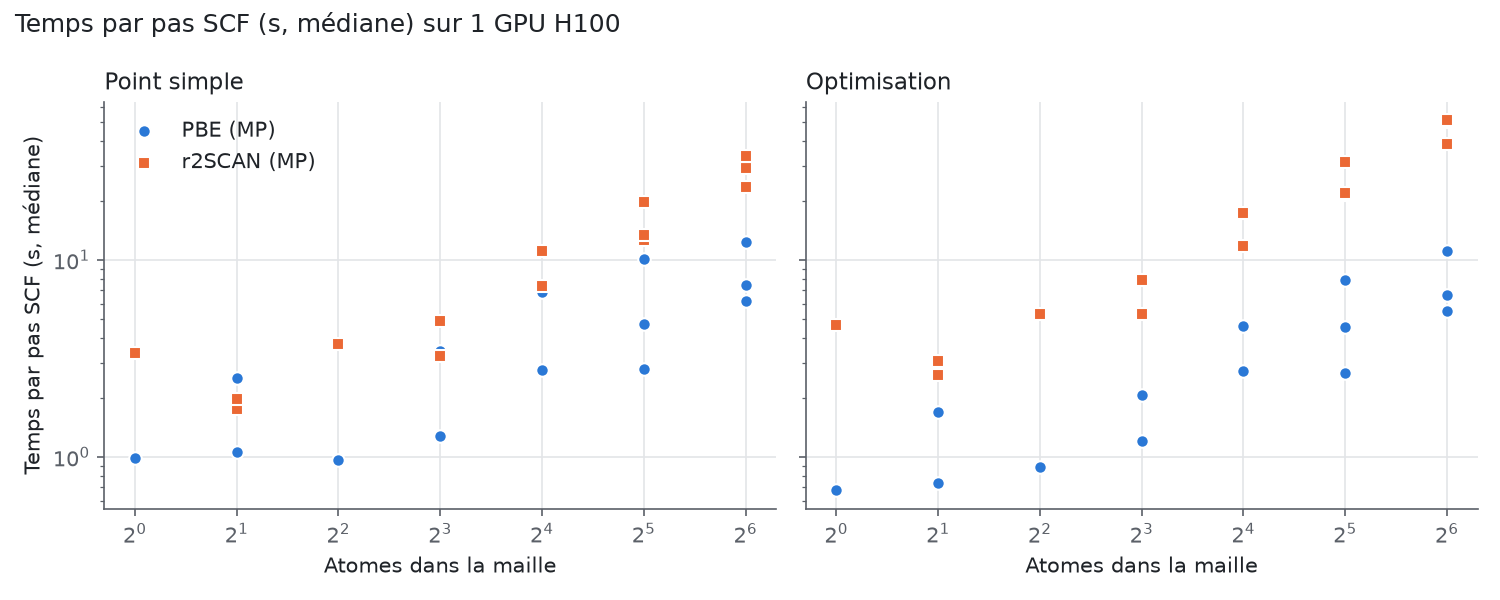
\includegraphics[width=0.78\linewidth]{t_scf_vs_natoms.png}
  \caption{Temps médian par pas SCF en fonction du nombre d'atomes, 1 GPU.}
  \label{fig:tscf}
\end{figure}

\subsection{Utilisation et mémoire}

\begin{itemize}
  \item \textbf{Utilisation moyenne} (fraction du temps où au moins un noyau tourne, relevée
        toutes les \SI{2}{s} par \texttt{nvidia-smi}) : 10 à \SI{50}{\percent} de 1 à 64 atomes.
        Cette mesure surestime l'occupation réelle : un noyau qui n'utilise qu'une partie des
        multiprocesseurs compte comme \og GPU occupée\fg.
  \item \textbf{Mémoire GPU} : environ \SI{2,9}{Go} dès un atome (contexte CUDA, bibliothèques,
        tableaux fixes de VASP), puis au plus \SI{5,2}{Go} en PBE et \SI{12,2}{Go} en \rscan{}
        (Al, 64 atomes, 12 points k). La mémoire n'est jamais une contrainte dans cette gamme.
  \item \textbf{Systèmes plus gros} : dans le scan de \texttt{NSIM}, l'utilisation atteint
        \SI{64}{\percent} pour Si 216 atomes et \SI{75}{\percent} pour LiN\textsubscript{3}
        144 atomes (8 points k), contre \SI{50}{\percent} pour MgO 32 atomes. La GPU commence
        à être bien employée vers 150--200 atomes.
\end{itemize}

\paragraph{Ce que cela veut dire.} Ces chiffres ne montrent pas que les H100 conviennent mal à
VASP ; ils montrent que des mailles de quelques dizaines d'atomes sont trop petites pour elles.
Toute la suite en découle : pour gagner du temps sur de petits systèmes, il faut surtout
\emph{remplir} la GPU, pas chercher à accélérer un calcul isolé.

% ---------------------------------------------------------------------------
\section{Coût des méthodes}
\label{sec:cout}

\subsection{\rscan{} par rapport à PBE}

Le tableau~\ref{tab:r2} compare les deux méthodologies MP telles qu'on les utilise : \rscan{}
cumule une fonctionnelle plus chère, une énergie de coupure plus haute (680 contre
\SI{520}{eV}) et parfois plus de points k (Al 64 atomes : 12 contre 3).

\begin{table}[htbp]
\centering
\caption{Rapport des temps \rscan{} / PBE sur 1 GPU, du plus petit au plus grand système de
chaque série.}
\label{tab:r2}
\small
\begin{tabular}{@{}l cccc@{}}
\toprule
 & \multicolumn{2}{c}{Point simple} & \multicolumn{2}{c}{Optimisation} \\
\cmidrule(lr){2-3}\cmidrule(l){4-5}
 & total & par pas SCF & total & par pas SCF \\
\midrule
Si (2 → 64 at.)  & 1,6 → 3,0 & 1,7 → 3,2 & 1,6 → 4,0 & 3,5 → 5,8 \\
Al (1 → 64 at.)  & 2,8 → 7,9 & 3,4 → 5,5 & 7,1 → 15,9 & 6,9 → 9,3 \\
MgO (2 → 64 at.) & 0,9 → 2,9 & 0,8 → 2,4 & 1,5 → 9,3 & 1,8 → 4,5 \\
\bottomrule
\end{tabular}
\end{table}

L'écart grandit avec la taille. En optimisation, \rscan{} demande en plus davantage de pas
ioniques (1 à 4) et SCF (13 à 46), car la maille s'ajuste à la nouvelle fonctionnelle à partir
de structures relaxées en PBE.

\subsection{HSE06}

Sur MgO 32 atomes (144 bandes, 12 points k), avec les mêmes réglages que le calcul PBE du scan
de \texttt{NSIM}, un pas électronique hybride HSE06 prend \SI{481}{} à \SI{487}{s}, contre
\SI{7,7}{s} en PBE : \textbf{environ 60 fois plus}. Un point simple HSE06 de 32 atomes
représente donc plusieurs heures de GPU ; c'est le domaine où le choix du nombre de points k
et des réductions de grille (\texttt{NKRED}) pèse le plus, bien plus que tout réglage de
parallélisation.

\subsection{Optimisation et point simple}

Les structures de départ étant déjà relaxées en PBE par MP, une optimisation PBE coûte 0,9 à
1,9 fois un point simple (1 à 3 pas ioniques). En \rscan{}, le rapport monte à 1,3--6,1, le
plus élevé pour MgO 64 atomes.

% ---------------------------------------------------------------------------
\section{Réglages de parallélisation}
\label{sec:parallelisation}

\subsection{Une ou deux GPU, et \texttt{KPAR}}

Les 56 calculs des séries d'échelle ont été refaits sur 2 GPU, avec les bandes réparties
(\texttt{KPAR} = 1) ou les points k répartis (\texttt{KPAR} = 2). Les énergies sont
identiques à celles sur 1 GPU (écart maximal \SI{0,01}{meV/atome}).

\begin{figure}[htbp]
  \centering
  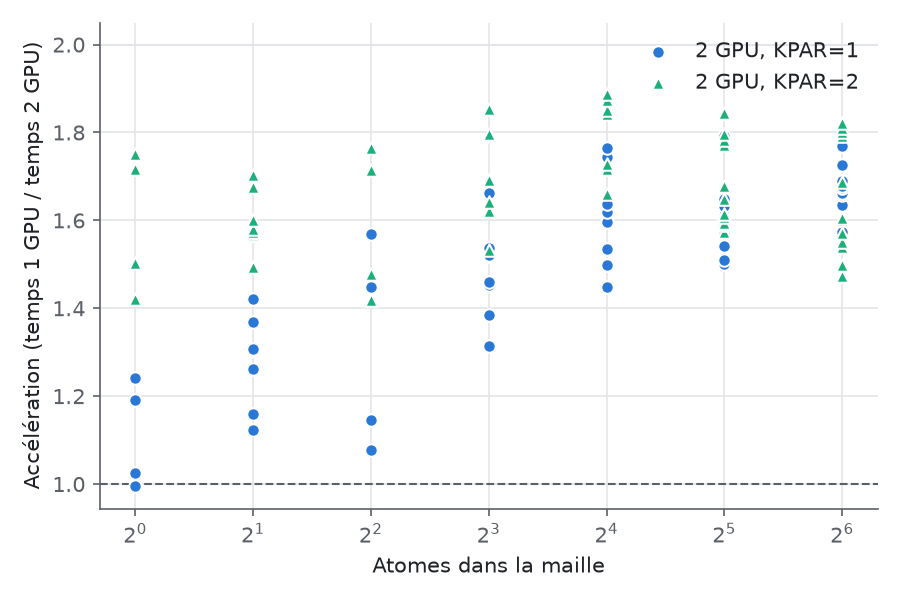
\includegraphics[width=0.78\linewidth]{speedup_2gpu.png}
  \caption{Accélération sur 2 GPU (temps sur 1 GPU / temps sur 2 GPU).}
  \label{fig:2gpu}
\end{figure}

\begin{itemize}
  \item \textbf{L'accélération est modeste} : 0,99 à 1,79$\times$ avec \texttt{KPAR} = 1,
        1,42 à 1,89$\times$ avec \texttt{KPAR} = 2. Deux GPU ne divisent jamais le temps
        par deux, alors que deux calculs indépendants, un par GPU, le font par construction.
  \item \textbf{\texttt{KPAR} = 2 est le bon choix par défaut} : plus rapide dans 42 cas sur
        56, notamment pour les petites mailles à nombreux points k (10 à 84), où répartir les
        bandes ne rapporte presque rien (Al 1 atome : 1,0$\times$ avec \texttt{KPAR} = 1).
  \item \textbf{\texttt{KPAR} = 1 ne gagne qu'à 64 atomes} avec 3 ou 4 points k (6 cas), en
        particulier quand les points k se répartissent mal (3 points : 2 + 1). Égalité à
        \SI{2}{\percent} près dans les 8 cas restants.
\end{itemize}

Pour les phonons, le temps VASP d'une chaîne complète passe de 0,5--\SI{1,7}{h} sur 1 GPU à
un temps 1,4 à 1,6 fois plus court sur 2 GPU, mais le coût en heures de GPU augmente de
25 à \SI{45}{\percent} (Si : 0,47 → \SI{0,58}{GPU\cdot h} ; MgO : 1,73 → \SI{2,52}{GPU\cdot h}).
Sur une machine partagée, l'attente d'une deuxième GPU libre a d'ailleurs allongé le temps de
restitution : \SI{8,1}{h} pour la campagne à 2 GPU contre \SI{6,0}{h} à 1 GPU.

\subsection{\texttt{NSIM} : aucun effet notable}

\texttt{NSIM} vaut 4 par défaut. On lit souvent qu'il faut l'augmenter sur GPU pour former de
plus grosses opérations matricielles. Deux campagnes indépendantes ont testé cette idée.

\paragraph{Scan de \texttt{NSIM} (4 à 128).} Travail électronique identique d'une valeur à
l'autre (nombre de pas imposé : 20 en PBE, 12 en HSE06), 1 GPU, une exécution par valeur.

\begin{table}[htbp]
\centering
\caption{Temps par pas électronique (s) selon \texttt{NSIM}, 1 GPU. Moyenne des pas après les
3 premiers (4 en HSE06). En gras : valeur la plus rapide. Dernière ligne de chaque bloc :
pic de mémoire GPU (Go).}
\label{tab:nsim}
\small
\begin{tabular}{@{}l l rrrrrr@{}}
\toprule
Système & & 4 & 8 & 16 & 32 & 64 & 128 \\
\midrule
MgO 32 at., PBE & s/pas & 7,90 & 7,70 & 7,68 & \textbf{7,67} & 7,77 & 7,68 \\
(144 bandes, 12 pts k) & Go & 4,7 & 4,8 & 4,9 & 5,1 & 5,5 & 5,9 \\
\addlinespace
LiN\textsubscript{3} 144 at., PBE & s/pas & 45,0 & 43,9 & 43,5 & 42,7 & \textbf{42,6} & 42,8 \\
(440 bandes, 8 pts k) & Go & 10,9 & 11,1 & 11,1 & 13,1 & 15,9 & 19,8 \\
\addlinespace
Si 216 at., PBE & s/pas & 19,8 & \textbf{19,6} & 19,7 & 19,7 & 20,3 & 20,8 \\
(606 bandes, point $\Gamma$) & Go & 12,1 & 12,7 & 14,7 & 18,0 & 24,2 & 39,3 \\
\addlinespace
MgO 32 at., HSE06 & s/pas & 483,6 & \textbf{481,1} & 483,2 & 486,6 & 484,4 & 486,5 \\
\bottomrule
\end{tabular}
\end{table}

\begin{figure}[htbp]
  \centering
  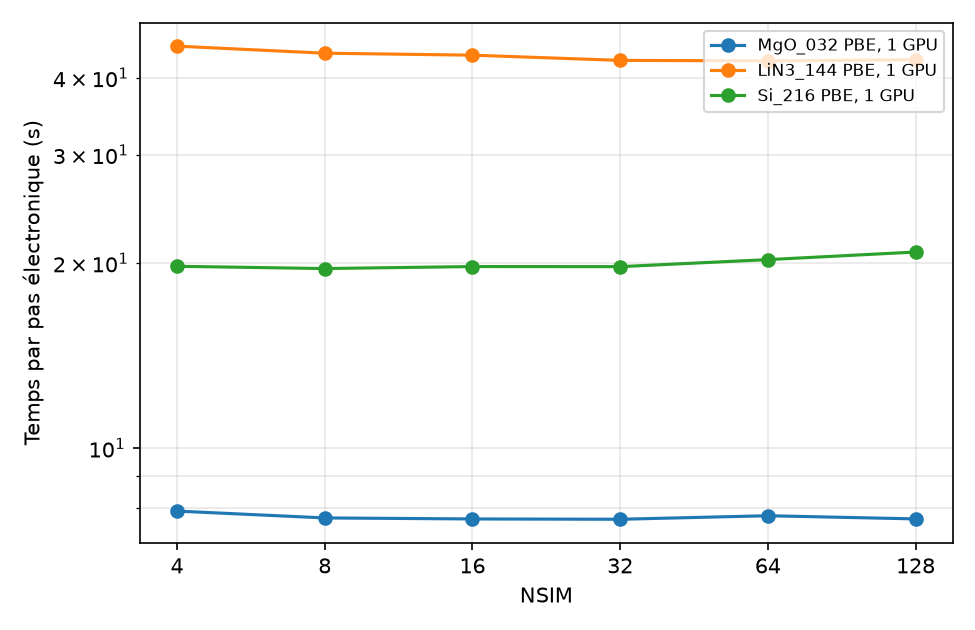
\includegraphics[width=0.72\linewidth]{nsim_time.png}
  \caption{Temps par pas électronique selon \texttt{NSIM}, PBE, 1 GPU (échelle logarithmique).}
  \label{fig:nsim}
\end{figure}

Le meilleur gain par rapport à \texttt{NSIM} = 4 est de \SI{3}{\percent} (MgO PBE),
\SI{6}{\percent} (LiN\textsubscript{3}), \SI{1}{\percent} (Si 216) et \SI{0,5}{\percent}
(HSE06). Pour Si 216 atomes, les grandes valeurs sont même nuisibles : $-$\SI{5}{\percent} à
\texttt{NSIM} = 128, avec une mémoire GPU multipliée par 3,2. Les énergies ne dépendent pas
de \texttt{NSIM} (écarts $\leq$ \SI{4e-5}{eV} par maille, dus à l'arrêt de la SCF après un
nombre fixe de pas). Réserve : les 18 calculs PBE ont tourné alors que d'autres jobs occupaient
le nœud ; les écarts de quelques pour cent sont du même ordre que cet effet.

\paragraph{Campagne test2 (\texttt{NSIM} = 32 contre 4).} Les 56 calculs 1 GPU des séries
d'échelle ont été refaits à l'identique, avec \texttt{NSIM} = 32 :
\begin{itemize}
  \item temps par pas SCF : rapport moyen (géométrique) de 1,005 ; médiane par série entre
        0,99 et 1,03 ; extrêmes 0,89 et 1,06 ;
  \item nombre de pas SCF identique dans 53 cas sur 56. Deux optimisations \rscan{} de MgO
        (32 et 64 atomes) sont 12 à \SI{16}{\percent} plus longues, mais par un chemin de
        convergence différent (39 → 44 pas SCF pour 32 atomes), pas par un pas plus lent ;
  \item énergies : écart maximal \SI{1,4e-4}{eV} par maille.
\end{itemize}

\paragraph{Conclusion sur \texttt{NSIM}.} Sur H100, de 2 à 216 atomes, en PBE, \rscan{} et
HSE06, \texttt{NSIM} ne modifie pas le temps de plus de quelques pour cent. Il n'y a pas lieu
de le régler ; si on le fait, rester entre 8 et 32 et éviter les grandes valeurs au point
$\Gamma$ sur de gros systèmes, qui coûtent de la mémoire sans rien rapporter.

\paragraph{Pourquoi \texttt{NSIM} ne change rien ici.} On lit couramment que, sur GPU, la
valeur par défaut \texttt{NSIM} = 4 sous-exploite la carte et qu'il faut passer à 16--32,
voire plus sur A100/H100. Nos mesures ne le confirment pas, et les OUTCAR permettent de
comprendre pourquoi :
\begin{enumerate}
  \item \textbf{La valeur demandée est bien appliquée} (\texttt{NSIM = 128} dans l'OUTCAR) :
        l'absence d'effet ne vient pas d'un paramètre ignoré.
  \item \textbf{La partie concernée domine pourtant le temps.} La mise à jour des orbitales
        (RMM-DIIS et Davidson, les routines où \texttt{NSIM} intervient) représente 92 à
        \SI{93}{\percent} de la boucle SCF pour LiN\textsubscript{3}, 78 à \SI{79}{\percent} pour
        Si 216 et \SI{99}{\percent} en HSE06. Passer de 4 à 64 ne réduit le temps RMM-DIIS de
        LiN\textsubscript{3} que de \SI{6}{\percent} (\SI{633}{} → \SI{597}{s}) ; pour Si 216,
        passer à 128 l'augmente de \SI{4}{\percent}.
  \item \textbf{Les noyaux sont déjà assez gros à \texttt{NSIM} = 4.} L'argument de
        l'occupation vaut pour des opérations trop petites. Or une seule transformée de Fourier
        sur la grille de Si 216 atomes ($126^3 \approx 2\times10^6$ points) offre déjà plus de
        travail parallèle qu'une H100 n'a de fils actifs à la fois (132 multiprocesseurs
        $\times$ 2048 fils $\approx 2{,}7\times10^5$). Les produits matriciels sur les bandes
        (orthogonalisation, diagonalisation dans le sous-espace) portent sur toutes les bandes
        et ne dépendent pas de \texttt{NSIM}. Grouper davantage de bandes n'apporte alors que
        des opérations plus grosses mais pas plus efficaces, et occupe plus de mémoire.
  \item \textbf{En HSE06}, le coût est celui de l'échange exact, calculé paire de bandes par
        paire de bandes et point k par point k ; \texttt{NSIM} n'agit pas sur ce
        regroupement.
\end{enumerate}
L'utilisation moyenne inférieure à \SI{100}{\percent} (50 à \SI{75}{\percent} dans ces calculs)
traduit plutôt des temps morts entre noyaux (lancements, synchronisations, parties restées sur
le CPU) que des noyaux trop petits, ce que \texttt{NSIM} ne peut pas corriger. Cette
explication reste à confirmer par un profilage (par exemple Nsight Systems) ; il est possible
que \texttt{NSIM} compte davantage pour des systèmes bien plus gros ou sur d'autres GPU. Les
recommandations générales trouvées dans la littérature restent valables sur un point,
confirmé ici : un \texttt{NSIM} élevé coûte de la mémoire GPU (Si 216 : \SI{12}{} →
\SI{39}{Go} de 4 à 128).

\subsection{\texttt{vasp\_gam} au point $\Gamma$}

Pour une AIMD de LiN\textsubscript{3} (144 atomes, point $\Gamma$ seul, PBE+D3, polarisé en
spin), \texttt{vasp\_gam}, qui exploite la symétrie réelle des fonctions d'onde, prend
\SI{61,2}{s} par pas ionique (13 pas SCF par pas, utilisation moyenne \SI{37}{\percent},
\SI{5,6}{Go}). Sur les 63 premiers pas, à trajectoire identique, \texttt{vasp\_std} prend
\SI{67,6}{s} par pas et \SI{7,7}{Go}. Le gain de \texttt{vasp\_gam} est donc d'environ
\SI{10}{\percent} en temps et \SI{27}{\percent} en mémoire : utile, sans plus. Mesure à confirmer sur 200 pas (le calcul
\texttt{vasp\_std} n'est pas allé au bout).

% ---------------------------------------------------------------------------
\section{Plusieurs calculs sur une même GPU : MPS}
\label{sec:mps}

Puisqu'un petit calcul laisse la GPU en grande partie inoccupée, on peut en lancer plusieurs
en même temps sur la même carte. Deux modes ont été comparés, avec N copies identiques d'un
point simple, dans un seul job Slurm, sans autre job sur le nœud :
\begin{itemize}
  \item \textbf{sans MPS} : chaque processus a son propre contexte CUDA et la GPU passe de l'un
        à l'autre par tranches de temps ;
  \item \textbf{avec MPS} (\emph{Multi-Process Service} de NVIDIA) : un serveur unique regroupe
        les processus, dont les noyaux s'exécutent réellement en même temps.
\end{itemize}

Gain de débit = $N \times t_\text{ref} / T_\text{lot}$, où $t_\text{ref}$ est le temps du
calcul seul et $T_\text{lot}$ celui du lot entier (idéal : $N$).

\begin{table}[htbp]
\centering
\caption{Gain de débit de N calculs simultanés sur une H100.}
\label{tab:mps}
\small
\begin{tabular}{@{}llr r cc cc cc@{}}
\toprule
 & & & & \multicolumn{2}{c}{N = 2} & \multicolumn{2}{c}{N = 4} & \multicolumn{2}{c}{N = 8} \\
\cmidrule(lr){5-6}\cmidrule(lr){7-8}\cmidrule(l){9-10}
Série & Composé & At. & $t_\text{ref}$ (s) & sans & MPS & sans & MPS & sans & MPS \\
\midrule
PBE SP & Si & 8 & 18 & 0,56 & 1,90 & 0,61 & 3,47 & 0,60 & \textbf{5,78} \\
PBE SP & MgO & 32 & 138 & 0,55 & 1,89 & 0,58 & 3,31 & 0,56 & \textbf{5,04} \\
\rscan{} SP & Al & 32 & 181 & 0,93 & 1,81 & 1,08 & 2,94 & 1,15 & \textbf{4,12} \\
\rscan{} SP & Si & 64 & 324 & 1,11 & 1,67 & 1,35 & \textbf{2,53} & -- & -- \\
\bottomrule
\end{tabular}
\end{table}

\begin{figure}[htbp]
  \centering
  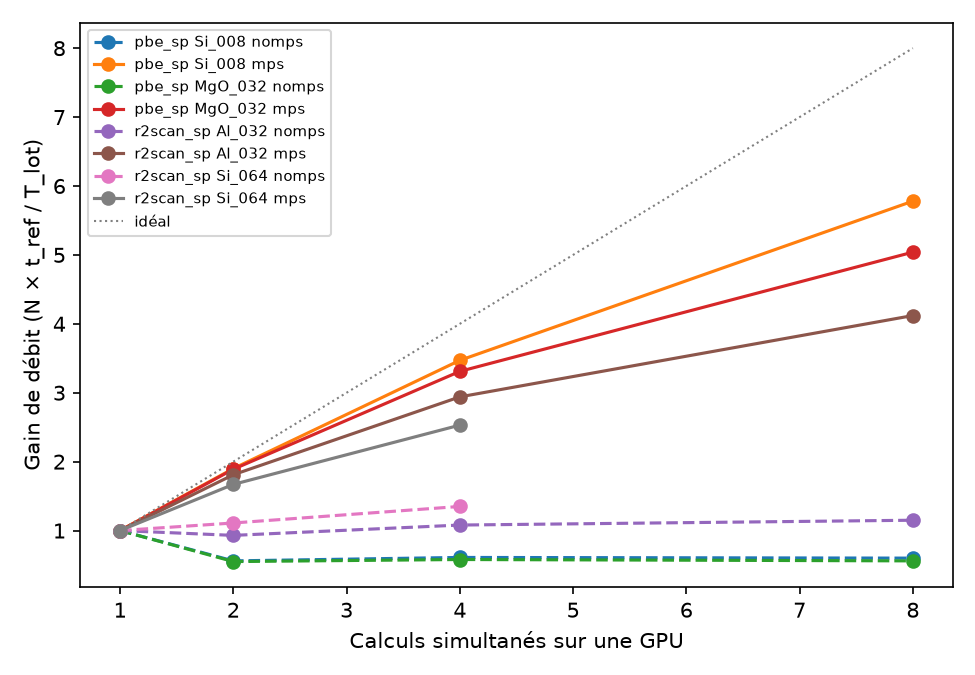
\includegraphics[width=0.72\linewidth]{concurrency_throughput.png}
  \caption{Gain de débit selon le nombre de calculs simultanés sur une GPU (tirets : sans MPS).}
  \label{fig:mps}
\end{figure}

\begin{itemize}
  \item \textbf{Avec MPS}, le débit est multiplié par 1,7--1,9 avec 2 calculs, 2,5--3,5 avec 4
        et 4,1--5,8 avec 8 ; chaque calcul n'est ralenti que de 1,3 à 1,9 fois à N = 8.
        L'utilisation moyenne passe de 25--\SI{37}{\percent} à 69--\SI{90}{\percent}.
  \item \textbf{Sans MPS}, c'est contre-productif : en PBE, le lot est 1,6 à 1,8 fois plus lent
        que les mêmes calculs lancés l'un après l'autre. Les changements de contexte coûtent
        plus que ce que l'on gagne.
  \item Le gain diminue quand la taille augmente : les plus petits calculs sont ceux qui
        laissent le plus de place libre.
  \item La limite pratique n'est pas la mémoire GPU (\SI{34,5}{Go} au plus pour 8 copies)
        mais la mémoire hôte allouée par Slurm (\SI{28}{Go} par GPU) : Si 64 atomes \rscan{}
        est limité à 4 copies.
  \item Les énergies des copies sont identiques à celle du calcul seul.
\end{itemize}

\paragraph{Mise en œuvre sur vm1-ic2mp.} Le démon MPS doit être démarré \emph{dans le job},
avec des répertoires privés, pour ne pas toucher aux autres utilisateurs. Extrait du script
\texttt{benchmark/run\_conc.slurm} :

\begin{lstlisting}[language=bash]
#SBATCH --gres=gpu:1
#SBATCH --ntasks=8
export OMP_NUM_THREADS=1
export CUDA_MPS_PIPE_DIRECTORY=/tmp/mps_${SLURM_JOB_ID}/pipe
export CUDA_MPS_LOG_DIRECTORY=/tmp/mps_${SLURM_JOB_ID}/log
mkdir -p "$CUDA_MPS_PIPE_DIRECTORY" "$CUDA_MPS_LOG_DIRECTORY"
nvidia-cuda-mps-control -d            # démarre le serveur MPS du job

PIDS=()
for c in calc-*; do                    # un dossier par calcul
    ( cd "$c" && mpirun -np 1 --bind-to none vasp_std > vasp.stdout 2>&1 ) &
    PIDS+=($!)
done
wait "${PIDS[@]}"                      # attendre ces PID-là, pas un « wait » nu

echo quit | nvidia-cuda-mps-control   # arrête le serveur MPS
rm -rf /tmp/mps_${SLURM_JOB_ID}
\end{lstlisting}

Le \texttt{wait} doit porter sur la liste des PID : un \texttt{wait} nu attendrait aussi un
éventuel moniteur \texttt{nvidia-smi} lancé en arrière-plan, et le job ne se terminerait jamais.

% ---------------------------------------------------------------------------
\section{Ordres de grandeur pour quelques flux de travail}
\label{sec:workflows}

\begin{center}
\small
\begin{tabular}{@{}p{0.45\linewidth}p{0.48\linewidth}@{}}
\toprule
Calcul (1 GPU) & Temps mesuré \\
\midrule
Point simple PBE, 1--64 atomes & 14 à \SI{163}{s} \\
Optimisation \rscan{}, 64 atomes & 12 min (Si) à 48 min (MgO) \\
Phonons PBE complets (relaxation, supercellules, Born) & \SI{0,5}{h} (Si), \SI{0,8}{h} (Al), \SI{1,7}{h} (MgO) \\
Point simple HSE06, MgO 32 atomes, 12 pas & \SI{1,3}{h} \\
AIMD PBE+D3, LiN\textsubscript{3} 144 atomes, \texttt{vasp\_gam} & \SI{61}{s} par pas de 1 fs : 200 pas en \SI{3,4}{h} ; 15 ps $\approx$ \SI{254}{h} \\
\bottomrule
\end{tabular}
\end{center}

Pour l'AIMD, le coût d'une trajectoire de plusieurs picosecondes justifie un champ de force
appris à la volée (MLFF de VASP) : la calibration correspondante est en attente de GPU au moment
de la rédaction et son gain reste à mesurer.

% ---------------------------------------------------------------------------
\section{Fiabilité des résultats}
\label{sec:fiabilite}

\begin{itemize}
  \item \textbf{Reproductibilité des temps} : sur 6 points simples répétés 3 fois, l'écart
        relatif du temps total ne dépasse pas \SI{1}{\percent}. Une différence de plus de
        quelques pour cent entre deux réglages est donc significative \emph{si} la machine
        est dans le même état ; d'autres jobs sur le nœud peuvent produire des écarts du même
        ordre.
  \item \textbf{Énergies} : identiques sur 1 et 2 GPU (\SI{0,01}{meV/atome}), quel que soit
        \texttt{KPAR} ou \texttt{NSIM}, et pour les calculs simultanés sous MPS.
  \item \textbf{Accord avec Materials Project} : à quelques meV/atome près, sauf deux cas
        compris (pseudopotentiel Mg plus ancien dans les données PBE de MP, $+$\SI{60}{meV/atome}
        constant ; échantillonnage en points k grossier de l'aluminium métallique en
        supercellule). Ces écarts ne viennent pas de la version GPU.
  \item \textbf{Phonons} : les fréquences obtenues sur 1 et 2 GPU diffèrent d'au plus
        \SI{5e-4}{THz}.
\end{itemize}

% ---------------------------------------------------------------------------
\section{Recommandations pratiques}
\label{sec:recommandations}

\begin{center}
\small
\begin{tabular}{@{}p{0.38\linewidth}p{0.56\linewidth}@{}}
\toprule
Situation & Réglage conseillé \\
\midrule
Un calcul jusqu'à $\sim$100 atomes & 1 GPU, 1 rang MPI, \texttt{OMP\_NUM\_THREADS} = 1 ;
ne pas toucher à \texttt{NSIM}. \\
\addlinespace
Beaucoup de petits calculs indépendants (criblage, déplacements de phonons, tests de
convergence) & 4 à 8 calculs par GPU sous MPS, démarré dans le job ; vérifier la mémoire hôte
($\leq$ \SI{28}{Go} par GPU). Jamais plusieurs calculs sur une GPU sans MPS. \\
\addlinespace
Un calcul urgent, assez gros & 2 GPU avec \texttt{KPAR} = 2 si le nombre de points k est
pair et $\geq$ 4 ; \texttt{KPAR} = 1 s'il n'y en a que 3 ou 4 et beaucoup de bandes.
Attendre au mieux un gain de 1,5 à 1,9. \\
\addlinespace
Point $\Gamma$ seul (grosses mailles, AIMD) & \texttt{vasp\_gam} : $-$\SI{10}{\percent} de
temps, $-$\SI{27}{\percent} de mémoire. \\
\addlinespace
Hybrides (HSE06) & Le coût ($\sim$60$\times$ PBE par pas) se joue sur les points k et
\texttt{NKRED}, pas sur \texttt{NSIM}. \\
\addlinespace
Dynamique moléculaire longue & Envisager un MLFF ; une AIMD pure de 144 atomes coûte
$\sim$\SI{17}{h} par picoseconde. \\
\addlinespace
Mesures de performance & Noter les autres jobs présents sur le nœud ; répéter au moins une
fois si l'écart attendu est inférieur à \SI{5}{\percent}. \\
\bottomrule
\end{tabular}
\end{center}

% ---------------------------------------------------------------------------
\section{Limites et suite}
\label{sec:limites}

\begin{itemize}
  \item \textbf{Pas de référence CPU} : seule la version GPU de VASP est installée sur le nœud ;
        aucune comparaison GPU / CPU n'est possible à partir de ces données.
  \item \textbf{Systèmes de taille moyenne} : l'essentiel des mesures porte sur 1 à 64 atomes ;
        seuls les scans de \texttt{NSIM} vont jusqu'à 144 et 216 atomes. Le domaine où la GPU
        est réellement remplie (plusieurs centaines d'atomes) reste à explorer.
  \item \textbf{Une seule exécution par valeur de \texttt{NSIM}}, en partie sur un nœud partagé.
  \item \textbf{AIMD et MLFF} : la calibration \texttt{vasp\_std} n'est pas terminée et les
        calculs MLFF n'ont pas encore tourné.
\end{itemize}

Suites prévues : production MLFF de LiN\textsubscript{3} (15 ps, 300 à 500 K), puis jeu de
diversité de 34 composés MP (points simples puis optimisations), qui élargira les conclusions
à des chimies variées et à des mailles jusqu'à 80 atomes.

\section*{Données et scripts}
Scripts, tableaux et figures sont dans le dépôt\\
\url{https://github.com/John-Akapulco/GPU_vmp_testing_VASP_etc} (dossiers \texttt{benchmark/}
et \texttt{benchmark/results/}). Rapport détaillé en anglais : \texttt{report/report.tex}.
Les sorties de VASP restent sur vm1-ic2mp.

\end{document}
